\documentclass{article}
\usepackage[utf8]{inputenc}

\usepackage{fullpage}

\usepackage{tikz}
%\usetikzlibrary{calc,arrows,shapes,backgrounds,patterns,fit,decorations,decorations.pathmorphing}

\usepackage[shadow,colorinlistoftodos,textwidth=2.5cm]{todonotes}
\usepackage[final,colorlinks,hyperindex,unicode=true,pdftitle=SPAdes Manual]{hyperref}
\usepackage{url}
\usepackage{booktabs}

\def\spades{SPAdes}

\usepackage{listings}
\definecolor{light-gray}{gray}{0.92}
\lstset{basicstyle=\ttfamily,framerule=0pt,frame=single,backgroundcolor=\color{light-gray}}

%\newenvironment{mycode}
%  {\begin{lstlisting}}
%  {\end{lstlisting}}

\begin{document}
\title{{\spades} Manual\\{\small Revision: \today}}
\date{}
\maketitle

%\begin{abstract}
{\spades} stands for St.~Petersburg genome assembler.
It is intended for both single cell and standard (multicell) 
assemblies. This manual will help you to install and run
{\spades}.


%\end{abstract}

\renewcommand{\contentsname}{}
\tableofcontents

%\pagebreak

%\listoftodos

\pagebreak

\section{General setting}
\subsection{Notation}
{\spades} works with paired end reads.
Read size, distance, gap, and insert length are 
explained in the picture below.

\begin{center}
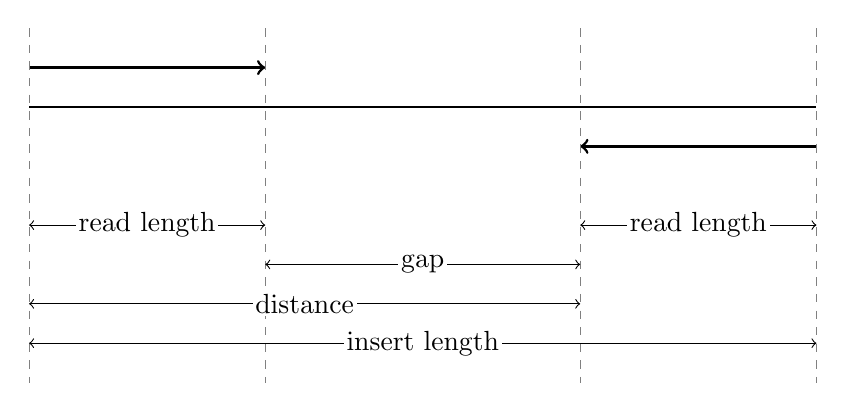
\begin{tikzpicture}
%\draw[help lines] (0,-3) grid (10,3);
\draw[line width=1pt] (0,2) -- (10,2);
\draw[line width=1pt,->] (0,2.5) -- (3,2.5);
\draw[line width=1pt,->] (10,1.5) -- (7,1.5);

\foreach \x in {0, 3, 7, 10}
  \draw[dashed,gray] (\x,3) -- (\x,-1.5);

\foreach \f/\s/\y/\t in {0/3/0.5/read length, 7/10/0.5/read length, 3/7/0/gap, 0/7/-0.5/distance, 0/10/-1/insert length}
\path[<->,draw] (\f,\y) -- node[fill=white,inner sep=1pt,rectangle] {\t} (\s,\y);
\end{tikzpicture}
\end{center}

\subsection{Config files and commands}
Config files and commands are given in gray boxes. 
Note that the text can be copy-pasted directly from this document.
%Note also that all the links and all the colored text in the manual are clickable.
In config files, parts of lines starting with a semicolon are just comments.


\section{Getting {\spades}}
The latest version of the source code can be downloaded from\\
\url{http://bioinf.spbau.ru/spades}\\
The following code shows how to download and unpack the archived file
directly from the command line.

\begin{lstlisting}
wget http://bioinf.spbau.ru/spades/spades.tar.gz
tar -xzf spades.tar.gz
\end{lstlisting}

\section{Requirements}\label{section:requirements}
\subsection{Packages}\label{subsection:packages}
%The following packages are required for using {\spades}.
The list of packages required for using {\spades} is given below.
The simplest way to install all of them is to run
\begin{lstlisting}
sudo ./install_prerequirements
\end{lstlisting}
This install all the required packages in a debian-like unix systems through {\tt apt-get install}.
If your operating system does not support {\tt apt-get} command you
need to install all the packages manually. 

\begin{center}
\begin{tabular}{lll}
\toprule
package & description & recommended version\\
\midrule
{\tt gcc++-4.4} & GNU C Compiler & 4.4\\
{\tt python2.6-dev} & Python & 2.6\\
% {\tt java-common} & Java & \\ % needed for quality
{\tt cmake} & make system & 2.6\\
{\tt liblog4cxx10-dev} & logging library for {\tt C++} & \\
{\tt libboost1.42-all-dev} & Boost {\tt C++} libraries & 1.42\\
{\tt zlib-bin} & compression library & \\
%%% the following libraries are needed for quality tool
%{\tt python-matplotlib} & plotting system & \\
%{\tt python-numpy} & fast arrays for python & \\
%{\tt bioperl} & Perl tools for computational molecular biology & \\
%{\tt mummer} & efficient sequence alignment of full genomes & \\
%{\tt r-recommended} & GNU R recommended packages & \\
%{\tt pdftk} & tool for manipulating PDF documents & \\
\bottomrule
\end{tabular}
\end{center}

\subsection{RAM}
It is recommended to run {\spades} on a $64$-bit linux system with at least $30$Gb of RAM.
E.g., on a multi-cell {\it E.coli} dataset {\spades} uses $20$Gb of RAM for error correction step
and $1.5$Gb of RAM for assembling.{\todo{Alexey, Sergey, are these the right estimates?}}

\section{Compiling}
When all the required packages are installed (see 
subsection~\ref{subsection:packages})
just run
\begin{lstlisting}
./preparecfg
\end{lstlisting}
in the root directory. 
This collects all dependencies and runs {\tt cmake}.

\section{Preparing input data}
\subsection{Correcting errors in your dataset}
\todo[inline]{Sergey Nikolenko, please fill in this subsection.}

\subsection{Adding your dataset to the config file}\label{subsec:datasets}
{\spades} requires paired end reads to be in separate files.
Additionally, {\spades} can use unpaired reads that normally appear after discarding one read of the paired read during error correction step.
Thus input reads should be arranged into four files: paired reads left parts, paired reads right parts, unpaired reads which originally were left parts, and
unpaired reads which originally were right parts. Thus, the first two files should contain the same number of reads, while
there are no requirements on the number of reads in the last two files (any of them can even be empty).
Files are expected to be in fasta or fastq formats and can be compressed.

In file {\tt configs/debruijn/datasets.info} add a new entry according to the following self-explaining pattern (recall that parts of lines starting from
semicolon are comments):{\todo{Misha, anything to be added here?}}
\begin{lstlisting}
ECOLI_IS220_QUAKE
{
  first            E.coli/s_6_1.fastq.gz ; paired left
  second           E.coli/s_6_2.fastq.gz ; paired right
  single_first     E.coli/s_6_1.single.fastq.gz ; unpaired left (optional)
  single_second    E.coli/s_6_2.single.fastq.gz ; unpaired right (optional)
  RL               100 ; read length
  IS               220 ; insert size (optional)
  variation        20 ; (optional)
  single_cell      false ; true if input data was obtained 
                         ; with mda (single cell) technology
  reference_genome E.coli/MG1655-K12.fasta.gz ; optional
}
\end{lstlisting}

\section{Running {\spades}}
To run {\spades} type
\begin{lstlisting}
./spades.py <config.info>
\end{lstlisting}
where {\tt <config.info>} contains all the parameters and looks like this.\todo{Valera, do not forget to rename output\_base =) }
\begin{lstlisting}
iterative_K         21 33 55
paired_mode         true 
dataset             ECOLI_IS220_QUAKE
input_dir           ./data/input/
output_dir         ./data/debruijn/
measure_quality     true
\end{lstlisting}

\begin{description}
\item[{\tt iterative\_K}] allows to set several $k$-mer sizes. Informally, smaller values of $k$ make graph more connected,
but at the same time more tangled, while higher values of $k$ may defragment the graph, but allow to resolve short repeats.
See the paper for more details.
\item[{\tt paired\_mode}] turns on/off the repeat resolver.
\item[{\tt dataset}] is the name of the dataset as it is given in {\tt configs/debruijn/datasets.info} (see subsection~\ref{subsec:datasets}).
\item[{\tt input\_dir}] is the directory where the corresponding dataset is stored.
\item[{\tt output\_dir}] is the output directory.
\item[{\tt measure\_quality}] flag allows to call quality estimation tool after the assembly is performed (the tool computes usual
metrics like N50, genome coverage, number of misassemblies, etc).
\end{description}

\section{Understanding the output}
Results can be found in {\tt data/debruijn/DATASET\_NAME/K.../DATE\_TIME}.
The specific directory is given at the end of the log, e.g.:
\begin{lstlisting}
289 ... Outputting contigs to ./data/debruijn/ECOLI_IS220_QUAKE/K55/
                                          01.16_19.05.28/contigs.fasta
289  INFO d (.../debruijn_stats.hpp:540) - Contigs written
290  INFO d (.../debruijn/launch.hpp:50) - Genome Assembling Finished
290  INFO d (.../debruijn/main.cpp:157) - Assembling ECOLI_IS220_QUAKE_1K 
                                          dataset finished
\end{lstlisting}

%The symlink {\tt latest} in the subfolder {\tt K...} leads to the latest run results folder.
%There are a lot of files there but the most important are the ones ending with {\tt .fasta}. Files {\tt before*} and {\tt after*} are contigs before 
%and after repeat resolution, respectively.

\section{FAQ}
\todo[inline]{Kira, Sonya, Yasha, what questions have you faced? =) }
%\subsection{How to choose the $k$-mer size?}
%\subsection{What if my question is not here?}



\end{document}
